\documentclass{article}
\usepackage{graphicx} % Required for inserting images

\title{DevOps - LLAMA GEMST}
\author{tbab, harw, gusm, edtr, mihr}
\date{May 2024}

\begin{document}

\maketitle

\section{Tasks}

\begin{itemize}
  \item Miha, Simon: security analysis — open
  \item Simon add a nice intro page
  \item Simon: find \& install template for latex file — more or less done — nice template lol
  \item Simon: look at Mircea's slides and make us a template for graphs — open for later
  \item finish Docker swarm — SH: fix fluendt 
    \item EDU: Implement Terrafrom
    \item Gustav: CD -> Create bash script to run the stack deploy
    \item EDU: Proxy after security is done, 21 km run
   \item Miha and Tomas: type

\subsection{DIAGRAMS}
 
    \item D1: layer distribution for cloud architecture 
    \item D2: General overview including everything 
    \item D2: Detailed overview CI/CD (pre commit: yaml file)
    \item D3: Detailed: Code architecture 
    \item D4: Detailed: Request diagrams for different stacks:
        \\ - -Grafana/Prometeus Stack: Quantitative 
        \\ - -EFK - Kibana/Elastic/Fluented: Qualitative

 \end{itemize}
\section{Introduction}
The following report described the work done during the Spring 2024 DevOps, Software Evolution and Software Maintenance taught at the IT University of Copenhagen. Our report includes the description of the final state of our system, the process we followed to develop and deploy it, lessons we learned, and reflections on technologies used and high and low level decisions we made throughout the semester.

\section{System's Perspective}
In this section, we describe the architecture of our ITU-MiniTwit system, the technologies that we used to support it, and we provide a rationale for the technologies we chose. This section also shows how a front-end or API request is processed by our system and what is eventually outputted. Finally, we show the results we obtained from using static analysis tools.

\subsection{How we refactored our app and why we chose GoLang. Tomas}

(note:include if you like it)
\begin{figure}[ht]
    \centering
    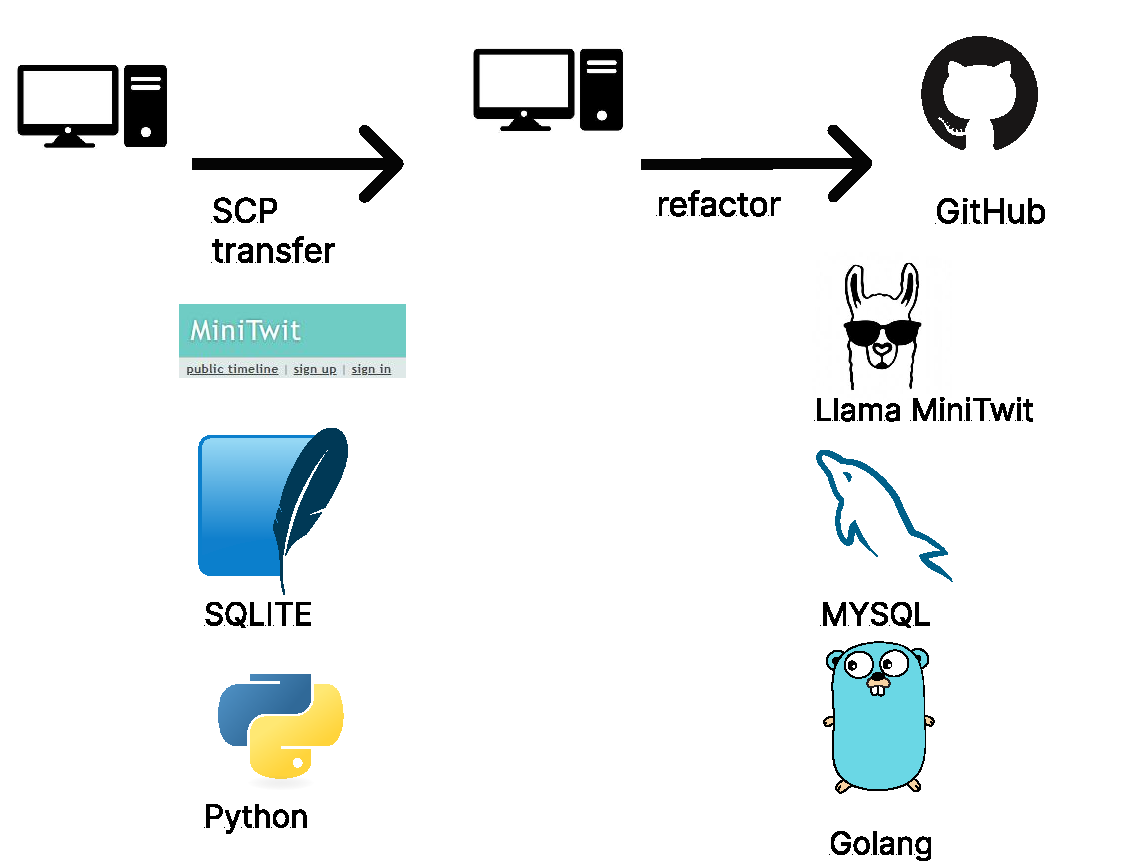
\includegraphics[width=0.8\textwidth]{./pdfs/refactoring.pdf} 
    \caption{MiniTwit refactoring}
    \label{fig:MiniTwit refactoring}
\end{figure}
I was thinking we can skip this paragraph. It's not that interesting in terms of DevOps to talk about translating an app into a new language and I already included "why we chose GO" in another paragraph :)
\\ -Go has numerous advantages related prone for code debugging
\\ -simplicity of the code =less typing compared to C
\\-good applications with cubanitas and docker
\\ -golang is open source which means continuous improvement and development.
\\-Golang is compiled and not interpreted language, which makes it very fast so we can see that it has better performance than Python
\\-Golang is designed to incorporate well concurrency (e.g. goroutine) unlike Python which can easily become a bottleneck for in concurrent tasks
\\-Python is consumes more memory compared to Golang which is more lightweight
\\-To run Python we are required to have python interpreter and related dependencies whereas Golang compiles to single binary without external
 dependencies
\\-benchmark comparison: Golang ~2-3ms vs Python ~21 ms
\subsection{How a request is processed when it comes from the front-end/simulator}
The following diagram shows how our system handles a request coming from the front-end or the API. We generally follow a model-view-controller architecture where the main function acts as the entry point of our application. Depending on the request type, the main function then forwards the request to handlers which redirect, handle logic, pass data to HTML templates or pass data to be written/read to/from the database. We chose this architecture as it would allow us to reuse code as much as possible and to seamlessly extend our code base. 
\\\\
For example, since we separated the methods that communicate with the database, we were able to add an abstraction layer without modifying the core logic of the application. Similarly, we were able to migrate our database from SQLite to a managed MySQL database on DigitalOcean very easily since our logic for connecting to the database was contained in one method which was invoked by several other methods when they needed to connect to the database.
\\\\
(Note: add D4 here)

\subsection{Architecture graphs of the system}

\subsection{Technologies used}
In this subsection we describe some of the key technologies we used on our system and justify them. The complete list of dependencies can be found in the appendix.

\subsubsection{Programming Languages}We chose to refactor our application using GoLang (Go). Go is a high level compiled programming language developed at Google in 2009. We chose to use it to refactor our app due to its simple syntax, automatic garbage collection and very high performance. Because of its easy to approach syntax, GoLang is generally regarded as a simple language to learn compared to others such as C++. For this reason, this made it a clear choice when we all saw the refactor of ITU-MiniTwit as an opportunity for our group members to learn a new language

note: shall we include the results from our benchmark?
\\\\
The automated tests that we used to monitor development on our app and make sure that no buggy code made it to our deployed application were written in Python. These were provided to us in the course repo and we chose not to refactor them to GoLang as we were able to use them to test our application.
\\\\
Finally, we used templated HTML files for the front-end of our application.

\subsubsection{Containerization and Orchestration Tools}
In order to ensure that our system had a high rate of availability (i.e. low down-time), we did horizontal scaling. Even though our cloud provider \textit{Digital Ocean} allows increasing droplet size (vertical scaling), we decided to also scale horizontally and thereby increase availability with \textit{Docker Swarm}. We chose this tool due to three reasons: 1) Ease of setup - since we already had experience with containerization \textit{Docker Swarm} was easy to pick up, 2) Load Balancing - \textit{Docker Swarm} has built-in load-balancing thereby increasing performance, and 3) Fault tolerance - by replicating nodes \textit{Docker Swarm} increases fault tolerance and availability.

\subsubsection{Database Technologies}
We were first provided with a lightweight SQLite database for ITU-MiniTwit. While this worked well for some time, we eventually realized that we needed a more persistent form of storage. We chose to purchase DigitalOcean's managed MySQL database solution. This was an easy choice for us as we were already using DigitalOcean to deploy our app online and using one of their database solutions allowed us to automatically refuse any incoming connection, except if it originated from our online application, which increased the security of our systems greatly. We also chose their MySQL solution as it was very easy to duplicate the schema used in the SQLite database that was provided to us and because we would be storing very structured data, eliminating the need for a document based database.
\\\\
In addition to this, we implemented a database-abstraction-layer via \textit{GORM}. This was done for several reasons:
\\\\
1) Since GORM supports multiple databases like SQLite, MySQL and PostgreSQL this added flexibility to our system since we were not tied to one single database for the entire cycle of our system.
\\\\
2) GORM provides auto-migration, which 
in short, makes it much easier to import an SQL table and perform operations on it. 


\subsection{Static Analysis Tool Results}
We gave two static analysis tools access to our GitHub repository: SonarCloud and CodeClimate. Both found some minor issues such as code smells, and maintainability issues, but did not raise any major problems such as bad code practices or security vulnerabilities. 
\\\\
\begin{figure}[ht]
    \centering
    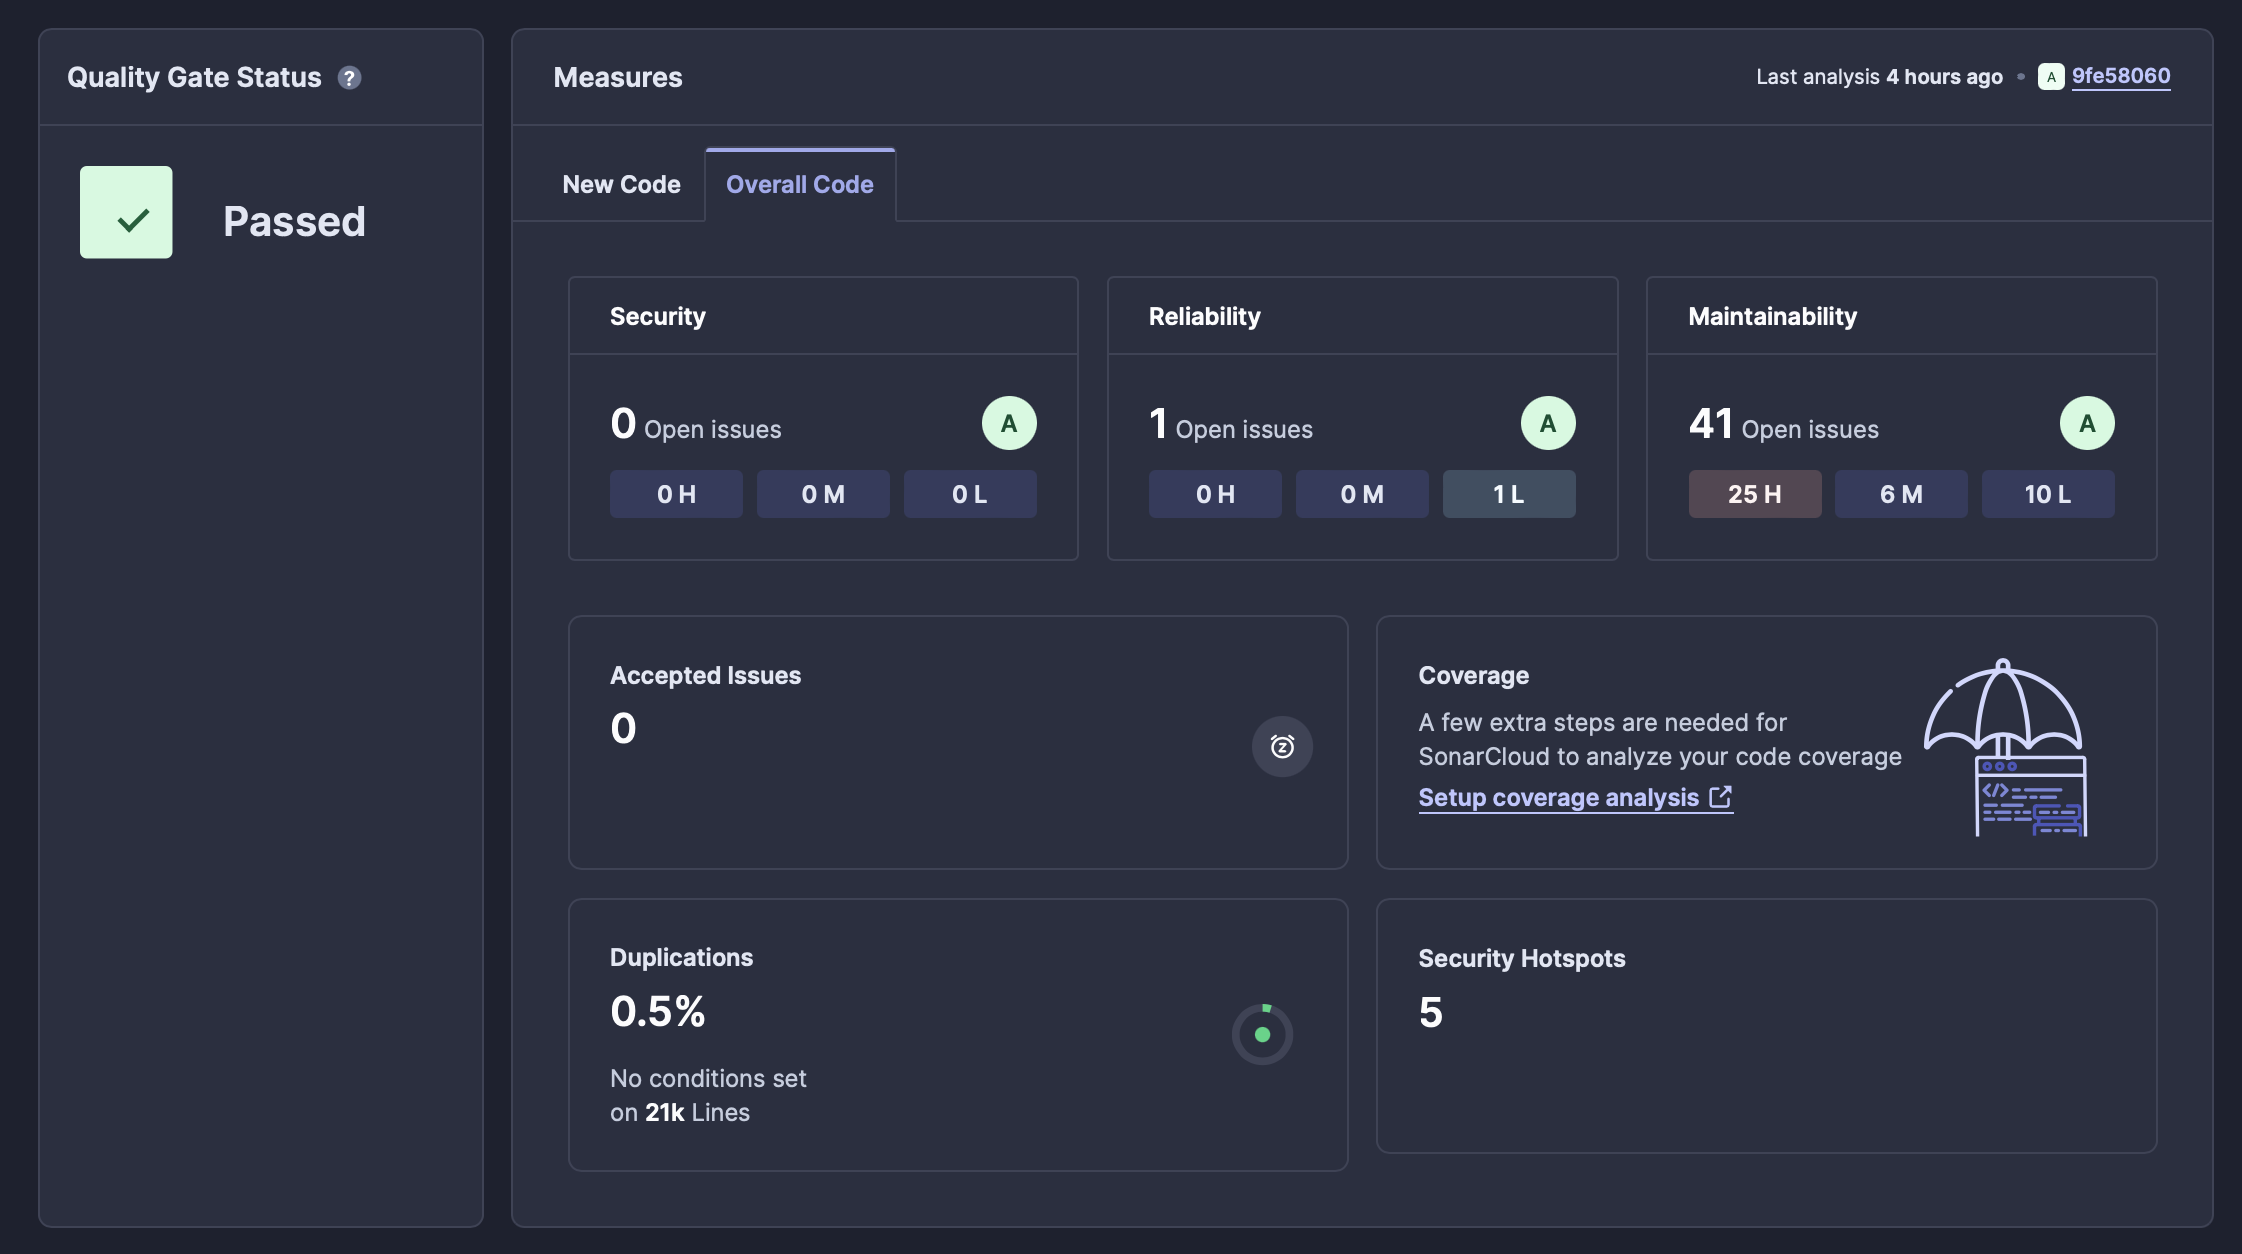
\includegraphics[width=0.8\textwidth]{./images/SonarCloud_Analysis.png}
    \caption{SonarCloud's dashboard after running an analysis on our repository.}
    \label{fig:notion-dashboard}
\end{figure}
\begin{figure}[ht]
    \centering
    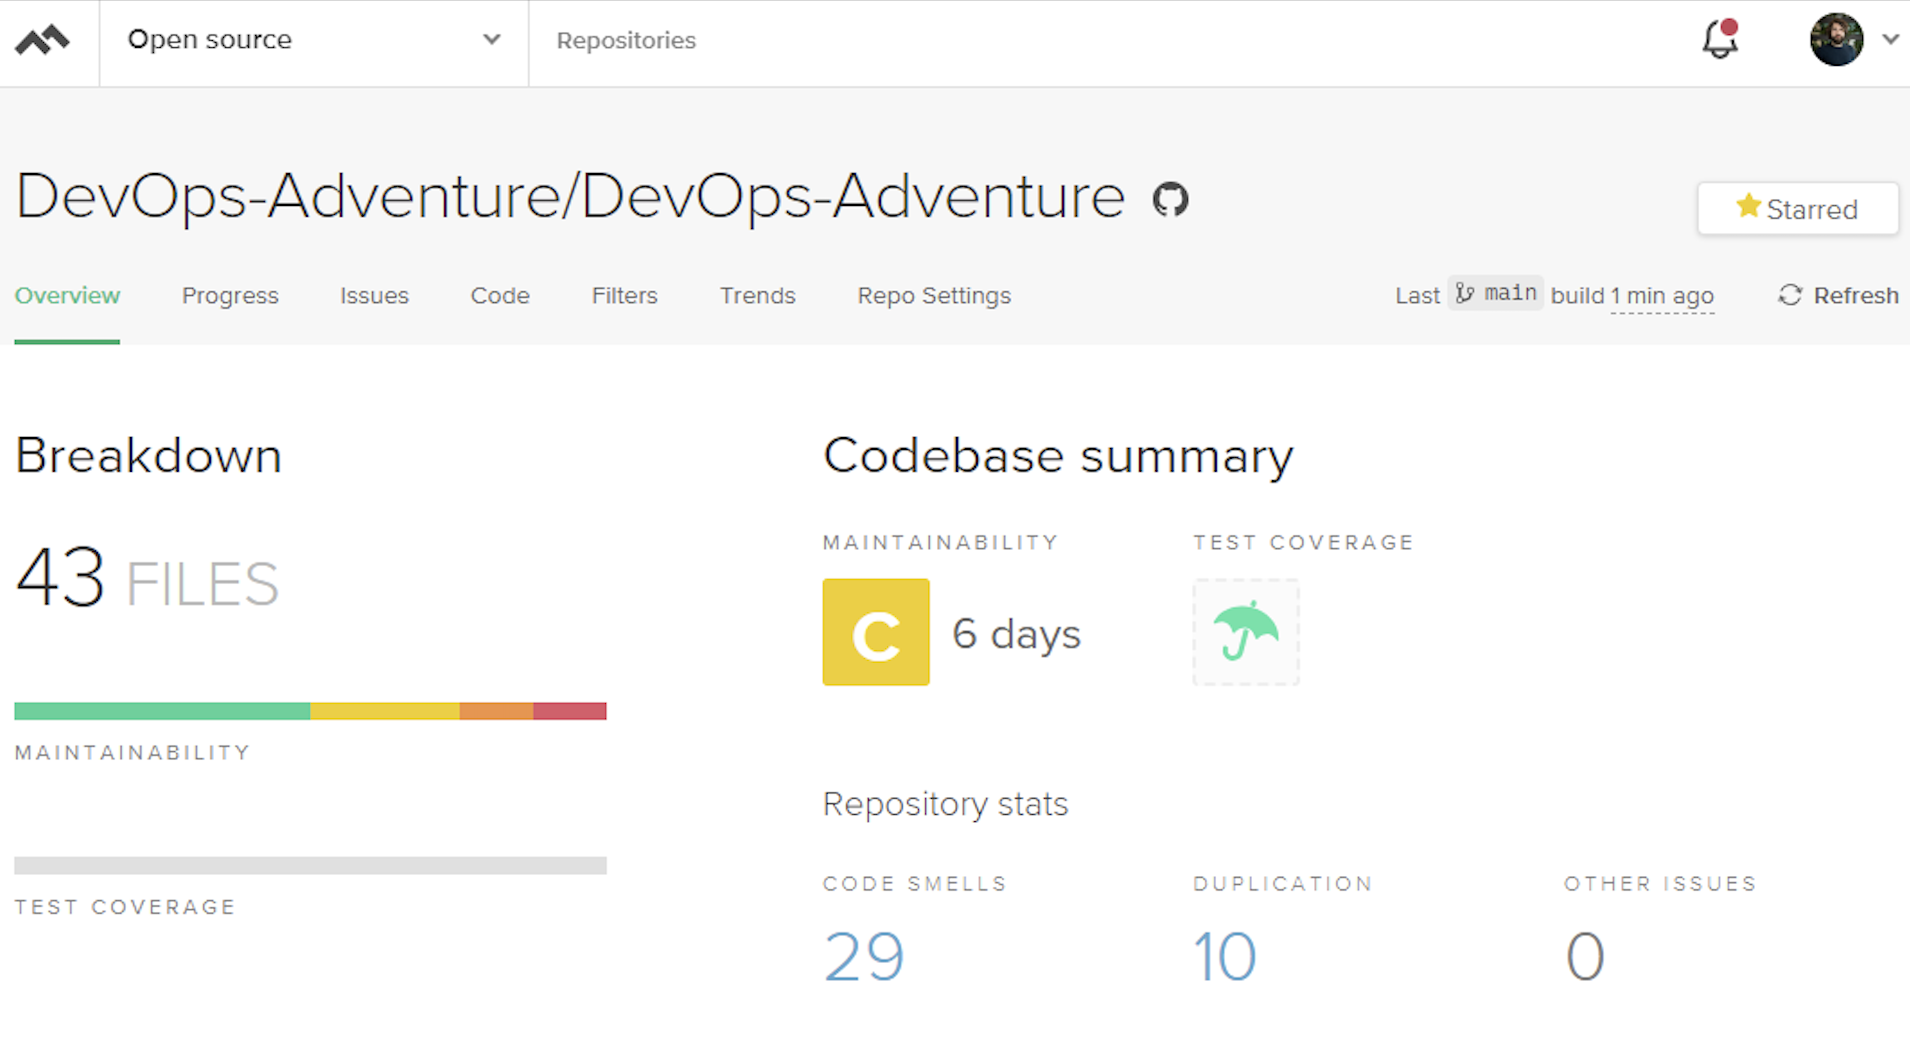
\includegraphics[width=0.8\textwidth]{./images/CodeClimate_analysis.png}
    \caption{Code Climate's dashboard after running an analysis on our repository.}
    \label{fig:notion-dashboard}
\end{figure}
\\\\
Furthermore, installing SonarCloud also gave us access to its bot which reviewed our code quality before we merged features into our main branch.
\\\\
\begin{figure}[ht]
    \centering
    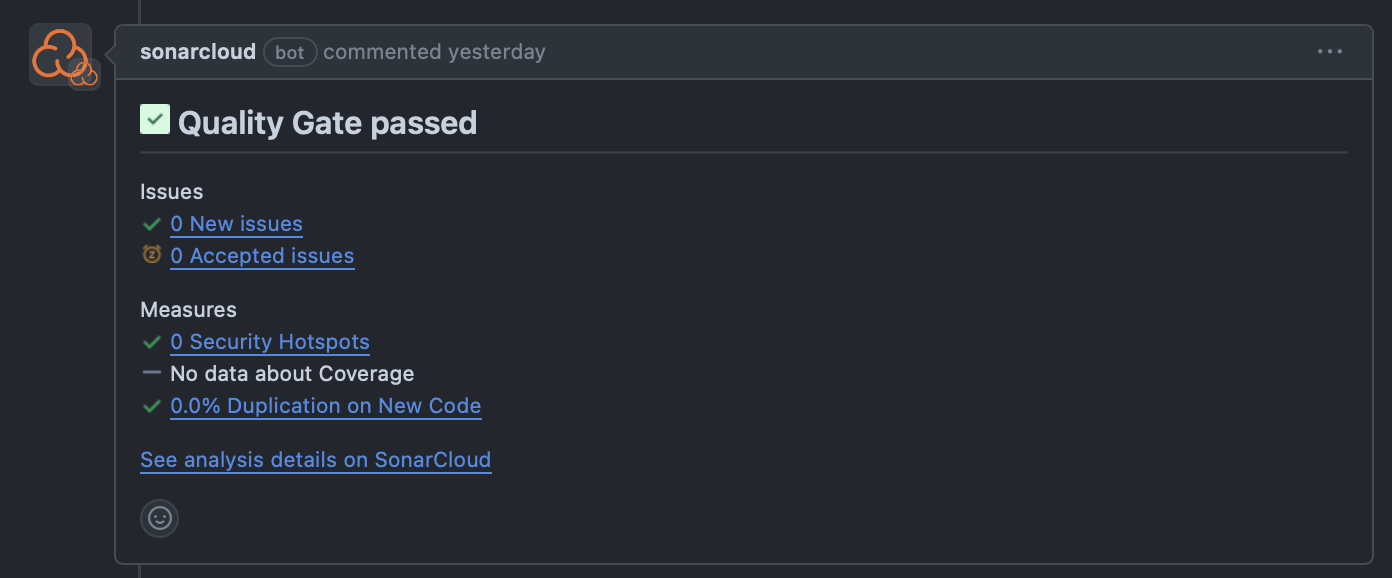
\includegraphics[width=0.8\textwidth]{./images/SonarCloud_bot.png}
    \caption{SonarCloud's bot adding comments on our pull requests.}
    \label{fig:notion-dashboard}
\end{figure}
\\\\

\section{Process' Perspective}

This perspective should clarify how code or other artifacts come from idea into the running system and everything that happens on the way.

In particular, the following descriptions should be included:

A complete description of stages and tools included in the CI/CD chains, including deployment and release of your systems.
How do you monitor your systems and what precisely do you monitor?
What do you log in your systems and how do you aggregate logs?
Brief results of the security assessment and brief description of how did you harden the security of your system based on the analysis
Applied strategy for scaling and upgrades
Also, in case you have used AI-assistants during your project briefly explain which system(s) you used during the project and reflect how it supported/hindered your process.

\subsection{Diagram showing our CI/CD chains, how we release and deploy MHR}

Stages and tools included in the CI/CD chains, including deployment and release;



\begin{figure}[ht]
    \centering
    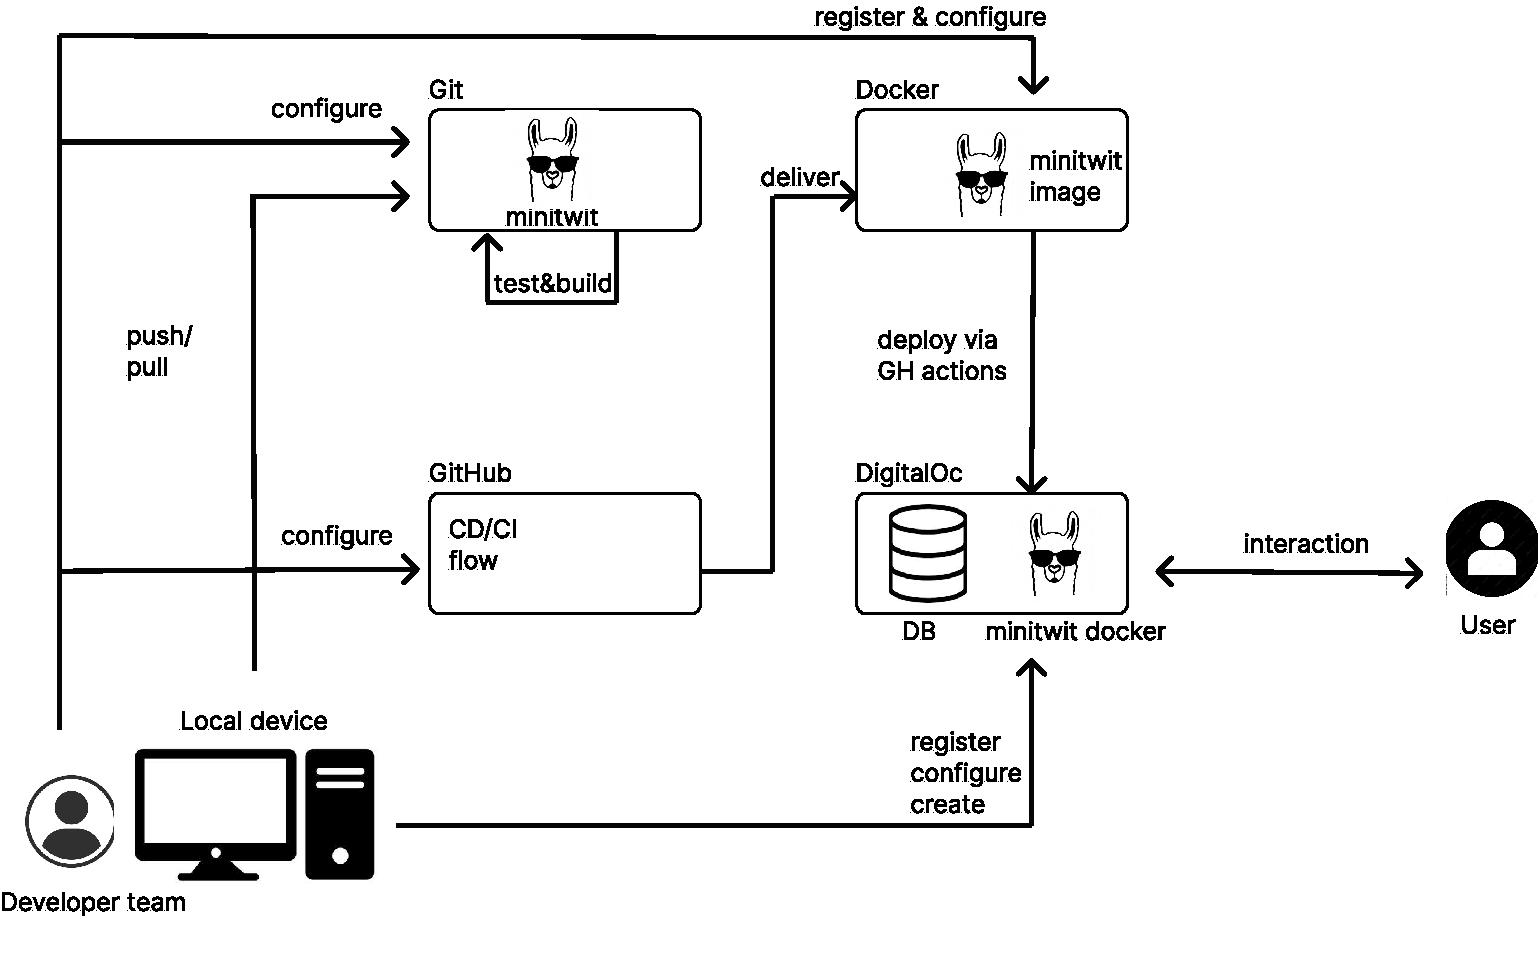
\includegraphics[width=0.8\textwidth]{./pdfs/CD-CI-flow.pdf} 
    \caption{CI/CD flow.}
    \label{fig:CD/CI flow}
\end{figure}

\subsection{How we used GIT}
Eduardo write this please
\subsection{How we monitor our systems and what we monitor/how we use this information to improve our system (give the example of indexing the db) MHR}

How do you monitor your systems and what precisely do you monitor?

Indexing:

\subsection{Logging and all that witchcraft crap. What we log and why we used those technologies, how we make sure that we're not logging too little but also not logging too much SIMON}
\subsection{Security assessment SIMON}
\subsection{Strategy for scaling and upgrading our system (talk about moving to a cloud db, and buying more droplets when moving to swarm}
\subsection{Our use of AI assistants MHR}

Chat GPT: for clarification of general knowledge
-useful when uploading error messages and suggestion for trying out different ways to solve the problem

 -useful to give simple examples that demonstrate the idea you want to implement

 -useful for getting quickly overview of how one function could work in different languages

 -not useful when asking for direct translation of one function to another

 -not useful when asking to provide direct answer

 Considerations for refactoring strategy:


\section{Lessons Learned Perspective}
In this section, we describe some of the technical and managerial difficulties we ran into during the semester, the lessons we learned from them and reflect on how we these difficulties could have been avoided or how we could have recovered more gracefully.

\subsection{Technical Issues}

\begin{itemize}
  \item Container being killed by the OS on the cloud
  \item Database cleared for some reason every now and then?
  \item Slow db querying (MHR)
  \item Swarm setup issues
\end{itemize}

\subsubsection{Resource Starvation}
During the 4th session of the course, we were tasked with deploying our ITU-MiniTwit system to the cloud so that the simulator could eventually interact with it through our API. We partitioned a droplet on DigitalOcean and deployed our app through a Docker container. We had a few additional services running on other containers but on the same droplet. Once the simulator started, our Docker container would seemingly randomly be shut down every few hours or every few days. After a few weeks of debugging, we eventually realized that there was a direct correlation between our container being shut off and when there was a spike in traffic on our ITU-MiniTwit. We quickly realized that the sum of the resources that we had allocated to each container running on the virtual machine installed on our droplet was higher than the resources we had purchased from Digital Ocean. More specifically, our containers were allowed to consume up to 6GB of RAM, but our droplet only provided us with 4. Thus, when the traffic spiked, the container consumed more RAM than it physically had access to and the OS would kill it.
\\\\
While it's easy for us to look back and recognize that this was a simple oversight, we had seen many tutorials that recommended capping the resources each Docker container could consume and had simply glanced over the information.

\subsection{Implementation of a CI/CD Pipeline, Automated Tests, and Good Git Practices}


\subsection{What tools we used during the semester, how we divided work, how we shared knowledge? MHR}

\subsection{The three DevOps ways and what we used?}

The Principles of Flow

\begin{itemize}

\item Make Work Visible
  \item Visibility:  In our group we apply the requirement of visibility in our work by defining and sharing our tasks in a common task board in Notion, bellow (by 03-03-2024). This helps us to keep track of the work that needs to be done and be informed what is each team member occupied with.

\begin{figure}[ht]
    \centering
    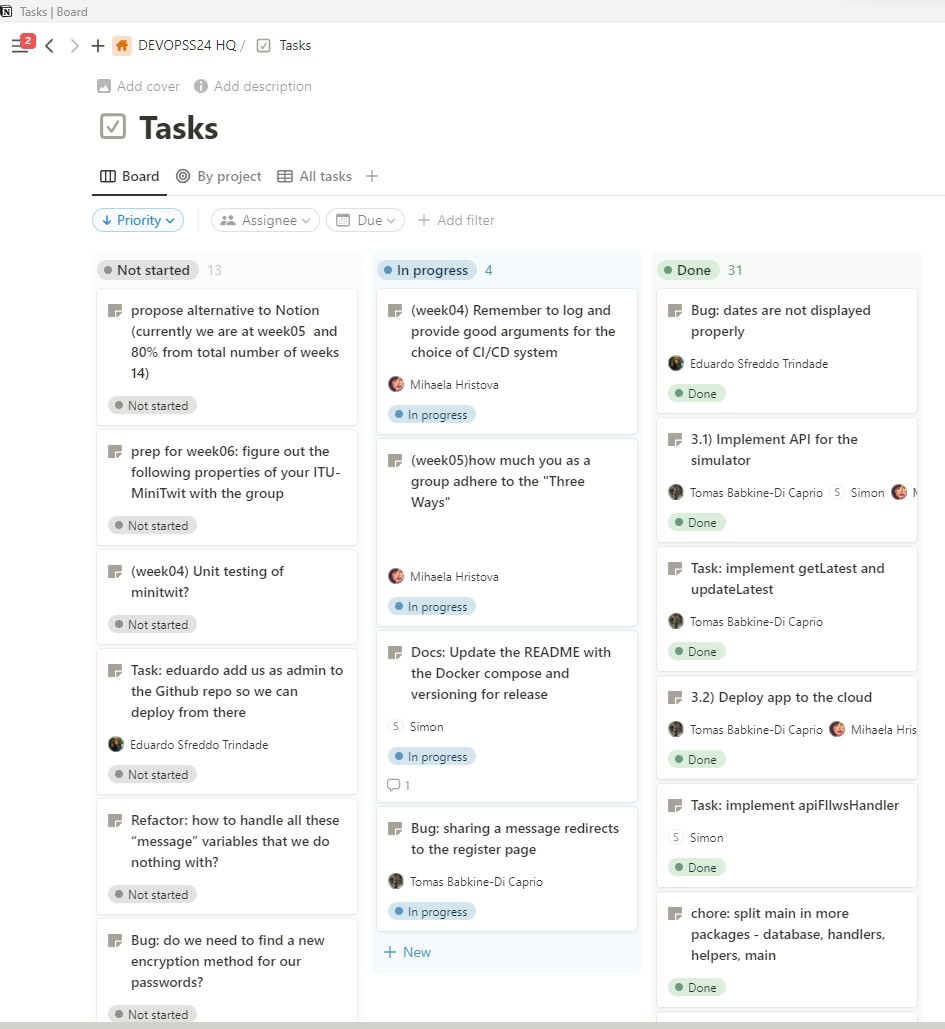
\includegraphics[width=0.8\textwidth]{./images/notion-dashboard-visibility-three-ways.png}
    \caption{Notion dashboard where we keep track of our tasks.}
    \label{fig:notion-dashboard}
\end{figure}
    
\item Limit Work in Progres
(to be implemented)

We have set a limit of the tasks  that can  be in each column in the Notion board) This means that we can only add a task when one is being finished. In case we are waiting on somebody’s task to be completed and we are free to start new task we will rather see what is causing the delay for our team member to finish his task and help him instead. 

here we could also implement a rule that new week cannot be started without completion of the task for the previous week OR having max three tasks that can be “carried” over.

\item  Reduce batch sizes:

in our case where we develop itu-minitwit application we could look at the different features for example post a message as a single unit operation that is being refactored, tested and deployed with the next *push* to main branch. The idea is instead of  trying to implement all features at once (post messages, follow user, register etc) we develop and test one at a time. This shortens the lead time significantly and most importantly help us to detect and act on bugs much faster.

\item  Reduce the number of hand-offs

Since we are a small organization that consist of 5 members we do not have a risk of wasting time on this principle. However we have implemented CI/CD flow that makes deployment to the cloud automated just with push to main branch. In out deployment process we use configured .yaml file “continuous deployment” that creates VM in Linus server, sets up a docker and tests out application in it (to be implemented), created a docker image of our application that sends to the server provider.

\item Continually Identify and Evaluate Constraints

improve work capacity by following the steps environment creation → code deployment → test setup and run → overly tight architecture

We have detached the dependency from local device by working with VM and Docker where we make sure that all needed requirements to run our application are present. Our deployment process is automated, that is consisted of automated testing of our application on Docker (to be implemented, Postman testing to be mentioned here perhaps? )

We have designed our app architecture with loose couples to achieve independency and safety when implementing changes.

\item Eliminate Hardships and Waste in the Value Stream

/using any material or resource beyond customer requirement is a waste/. Categories of waste: 

-partially done work: all team members are responsible for completion of the task assigned. Even they happen to need help in completion, the initially assigned person has to keep track of the status of the task.

-extra processes: we follow the mandatory assignments that are release each week without trying to develop unrequested features or any other way of deviating of project course work

-extra features: look above

-task switching: we try to keep one person for a task, in case the task is more difficult we might assign more than one person. We do not assign a person to multiple task in case he is unable to complete at least one of them.

-waiting: in case we need to wait for a member to complete his task we always offer help and accelerate the process.

-motion: we meet regularly in person for our lectures and we make sure to have at least one meeting in person per week. When we are not co-located we are distributing our tasks accordingly. Person that is not present gets rather independent task and vise versa. 

-defects: we make sure to be completely informed for a task before we take over.

-nonstandard or manual work: we make sure that nobody is using non-rebuilding servers, test environments and configuration. All our dependencies and operations are aimed to be automatic, self-services and available on demand.

-heroics: unfortunately we cannot ensure that all of our work is happening smoothly and often we depend on each other. This is a common scenario when we have to implement operation or a feature that we are all unexperienced in and we might need another member to give us a green light - for example we have enabled revision/review of the code in our gitHub that requires at least one more member to accept review of the code before we are able to merge. We work on a separate branch each week that is being merged before submission. In case of debug on the main ( for example when implementing CI/CD frow) that required multiple PR and therefore someone else on a stand by to accept the review request (in the middle of the night).

\item REFERENCES

1. Official website of Go https://go.dev/
-for installation and tutorials

2. LinkedIn learning “Learning Go” by David Gassner
https://www.linkedin.com/learning/learning-go-8399317/explore-go-s-variable-types?u=55937129


\end{itemize}

\end{document}